\documentclass[a4paper,12pt]{report}

\usepackage{setspace}
\onehalfspacing


%%% Поля и разметка страницы %%%
\usepackage{lscape}		% Для включения альбомных страниц
\usepackage{geometry}	% Для последующего задания полей

%%% Кодировки и шрифты %%%
\usepackage{cmap}						% Улучшенный поиск русских слов в полученном pdf-файле
\usepackage[T2A]{fontenc}				% Поддержка русских букв
\usepackage[utf8]{inputenc}				% Кодировка utf8
\usepackage[english, russian]{babel}	% Языки: русский, английский
\usepackage{hhline}	
\usepackage{lastpage}

%%% Математические пакеты %%%
\usepackage{amsthm,amsfonts,amsmath,amssymb,amscd} % Математические дополнения от AMS

%%% Оформление абзацев %%%
\usepackage{indentfirst} % Красная строка

%%% Цвета %%%
\usepackage[usenames]{color}
\usepackage{color}

%%% Таблицы %%%
\usepackage{longtable}					% Длинные таблицы
\usepackage{multirow,makecell,array}	% Улучшенное форматирование таблиц

%%% Общее форматирование
\usepackage[singlelinecheck=off,center]{caption}	% Многострочные подписи
\usepackage{soul}									% Поддержка переносоустойчивых подчёркиваний и зачёркиваний

%%% Библиография %%%
\usepackage{cite} % Красивые ссылки на литературу

\usepackage{ifthen}                 % добавляет ifthenelse

% настройка подписей к рисункам и таблицам
\usepackage{caption}
\usepackage{subcaption}

%%% Гиперссылки %%%
\usepackage[linktocpage=true,plainpages=false,pdfpagelabels=false]{hyperref}

%%% Изображения %%%
\usepackage{graphicx} % Подключаем пакет работы с графикой

%%% Оглавление %%%
\usepackage{tocloft}

%%% Подписи %%%
\usepackage{caption}                                % Для управления подписями (рисунков и таблиц) % Может управлять номерами рисунков и таблиц с caption %Иногда может управлять заголовками в списках рисунков и таблиц
\usepackage{subcaption}                             % Работа с подрисунками и подобным

\usepackage{textcomp}
\usepackage{calc}

\usepackage{titlesec} % для titleformat
\usepackage{interfaces-base}

% для номеров страниц
\usepackage{fancyhdr} % пакет для установки колонтитулов

%%% Счётчики %%%
\usepackage[figure,table]{totalcount}               % Счётчик рисунков и таблиц
\usepackage{totcount}                               % Пакет создания счётчиков на основе последнего номера подсчитываемого элемента (может требовать дважды компилировать документ)

%\usepackage{todonotes}

\RequirePackage{keyval}
\usepackage{ifthen}

\usepackage{amsmath,amssymb}
\usepackage{enumitem}
\usepackage{textpos}

		% Подключаемые пакеты
\LoadInterface{titlesec}                   % Подгружаем интерфейсы для дополнительных опций управления некоторыми пакетами

%%% Макет страницы %%%
\geometry{a4paper,top=1cm,bottom=2.3cm,left=2.5cm,right=0.7cm}

\setlength{\footskip}{43pt}


%%% Кодировки и шрифты %%%
\renewcommand{\rmdefault}{ftm} % Включаем Times New Roman

%%% Выравнивание и переносы %%%
\sloppy					% Избавляемся от переполнений
\clubpenalty=10000		% Запрещаем разрыв страницы после первой строки абзаца
\widowpenalty=10000		% Запрещаем разрыв страницы после последней строки абзаца

%\linespread{1.3}

%%% Изображения %%%
\graphicspath{{images/}} % Пути к изображениям

\usepackage{amsmath}
\newcommand{\argmax}{\operatornamewithlimits{arg\ max}}

% для жирных греческих букв
\usepackage{bm}


%%% Колонтитулы %%%
% Порядковый номер страницы печатают на середине верхнего поля страницы (ГОСТ Р 7.0.11-2011, 5.3.8)
\makeatletter
\let\ps@plain\ps@fancy              % Подчиняем первые страницы каждой главы общим правилам
\makeatother
\pagestyle{fancy}                   % Меняем стиль оформления страниц
\fancyhf{}                          % Очищаем текущие значения


\renewcommand{\headrulewidth}{0pt}  % Убираем разделительную линию

\newcounter{headingalign}
\newcounter{otstup}
\newcounter{pgnum}

%% Выравнивание заголовков в тексте
\setcounter{headingalign}{0}        % 0 --- по центру; 1 --- по левому краю

%% Отступы у заголовков в тексте
\setcounter{otstup}{1}              % 0 --- без отступа; 1 --- абзацный отступ

%%% Блок управления параметрами для выравнивания заголовков в тексте %%%
\newlength{\otstuplen}
\setlength{\otstuplen}{\theotstup\parindent}
\ifthenelse{\equal{\theheadingalign}{0}}{% выравнивание заголовков в тексте
	\newcommand{\hdngalign}{\filcenter}                % по центру
	\newcommand{\hdngaligni}{\hfill\hspace{\otstuplen}}% по центру
}{%
\newcommand{\hdngalign}{\filright}                 % по левому краю
\newcommand{\hdngaligni}{\hspace{\otstuplen}}      % по левому краю
} % В обоих случаях вроде бы без переноса, как и надо (ГОСТ Р 7.0.11-2011, 5.3.5)

%%% Оформление заголовков глав, разделов, подразделов %%%
%% Работа должна быть выполнена ... размером шрифта 12-14 пунктов (ГОСТ Р 7.0.11-2011, 5.3.8). То есть не должно быть надписей шрифтом более 14. Так и поставим.
%% Эти установки будут давать одинаковый результат независимо от выбора базовым шрифтом 12 пт или 14 пт
\titleformat{\chapter}[block]                                % default display;  hang = with a hanging label. (Like the standard \section.); block = typesets the whole title in a block (a paragraph) without additional formatting. Useful in centered titles
{\hdngalign\fontsize{12pt}{16pt}\selectfont\bfseries}% 
%\fontsize{<size>}{<skip>} % второе число ставим 1.2*первое, чтобы адекватно отрабатывали команды по расчету полуторного интервала (домножая разные комбинации коэффициентов на этот)
{\thechapter\cftchapaftersnum}                       % Заголовки в оглавлении должны точно повторять заголовки в тексте (ГОСТ Р 7.0.11-2011, 5.2.3).
{0em}% отступ от номера до текста
{}%

\titleformat{\section}[block]                                % default hang;  hang = with a hanging label. (Like the standard \section.); block = typesets the whole title in a block (a paragraph) without additional formatting. Useful in centered titles
{\hdngalign\fontsize{12pt}{16pt}\selectfont\bfseries}% 
%\fontsize{<size>}{<skip>} % второе число ставим 1.2*первое, чтобы адекватно отрабатывали команды по расчету полуторного интервала (домножая разные комбинации коэффициентов на этот)
{\thesection\cftsecaftersnum}                        % Заголовки в оглавлении должны точно повторять заголовки в тексте (ГОСТ Р 7.0.11-2011, 5.2.3).
{0em}% отступ от номера до текста
{}%

\titleformat{\subsection}[block]                             % default hang;  hang = with a hanging label. (Like the standard \section.); block = typesets the whole title in a block (a paragraph) without additional formatting. Useful in centered titles
{\hdngalign\fontsize{12pt}{16pt}\selectfont\bfseries}% 
%\fontsize{<size>}{<skip>} % второе число ставим 1.2*первое, чтобы адекватно отрабатывали команды по расчету полуторного интервала (домножая разные комбинации коэффициентов на этот)
{\thesubsection\cftsubsecaftersnum}                  % Заголовки в оглавлении должны точно повторять заголовки в тексте (ГОСТ Р 7.0.11-2011, 5.2.3).
{0em}% отступ от номера до текста
{}%

\newcounter{chapstyle}
\setcounter{chapstyle}{1}           % 0 --- разделы только под номером; 1 --- разделы с названием "Глава" перед номером

\ifthenelse{\equal{\thechapstyle}{1}}{%
	\sectionformat{\chapter}{% Параметры заголовков разделов в тексте
		label=\chaptername\ \thechapter\cftchapaftersnum,
		labelsep=0em,
	}
}

\newcounter{headingdelim}
\setcounter{headingdelim}{2}        % 0 --- номер отделен пропуском в 1em или \quad; 1 --- номера разделов и приложений отделены точкой с пробелом, подразделы пропуском без точки; 2 --- номера разделов, подразделов и приложений отделены точкой с пробелом.

%\DeclareCaptionLabelSeparator*{emdash}{.}             % (ГОСТ 2.105, 4.3.1)
\captionsetup[figure]{labelformat=simple,labelsep=period,position=bottom}
\captionsetup[table]{labelformat=simple,labelsep=period,position=bottom}


%%% Оглавление %%%
\renewcommand{\cftchapdotsep}{\cftdotsep}                % отбивка точками до номера страницы начала главы/раздела
\renewcommand{\cfttoctitlefont}{\hdngaligni\fontsize{14pt}{16pt}\selectfont\bfseries}% вместе со следующей строкой
\renewcommand{\cftaftertoctitle}{\hfill}                 % устанавливает заголовок по центру

%% Переносить слова в заголовке не допускается (ГОСТ Р 7.0.11-2011, 5.3.5). Заголовки в оглавлении должны точно повторять заголовки в тексте (ГОСТ Р 7.0.11-2011, 5.2.3). Прямого указания на запрет переносов в оглавлении нет, но по той же логике невнесения искажений в смысл, лучше в оглавлении не переносить:
\cftsetrmarg{2.55em plus1fil}                       %To have the (sectional) titles in the ToC, etc., typeset ragged right with no hyphenation
\renewcommand{\cftchappagefont}{\normalfont}        % нежирные номера страниц у глав в оглавлении
\renewcommand{\cftchapleader}{\cftdotfill{\cftchapdotsep}}% нежирные точки до номеров страниц у глав в оглавлении
%\renewcommand{\cftchapfont}{}                       % нежирные названия глав в оглавлении

\ifthenelse{\theheadingdelim > 0}{%
	\renewcommand\cftchapaftersnum{.\ }   % добавляет точку с пробелом после номера раздела в оглавлении
}{%
\renewcommand\cftchapaftersnum{\quad}     % добавляет \quad после номера раздела в оглавлении
}
\ifthenelse{\theheadingdelim > 1}{%
	\renewcommand\cftsecaftersnum{.\ }    % добавляет точку с пробелом после номера подраздела в оглавлении
	\renewcommand\cftsubsecaftersnum{.\ } % добавляет точку с пробелом после номера подподраздела в оглавлении
}{%
\renewcommand\cftsecaftersnum{\quad}      % добавляет \quad после номера подраздела в оглавлении
\renewcommand\cftsubsecaftersnum{\quad}   % добавляет \quad после номера подподраздела в оглавлении
}

			% Пользовательские стили
\usepackage{eso-pic}

\newcommand\BackgroundPic{
	\put(0,0){
		\parbox[b][\paperheight]{\paperwidth}{%
		\vfill
		\centering
		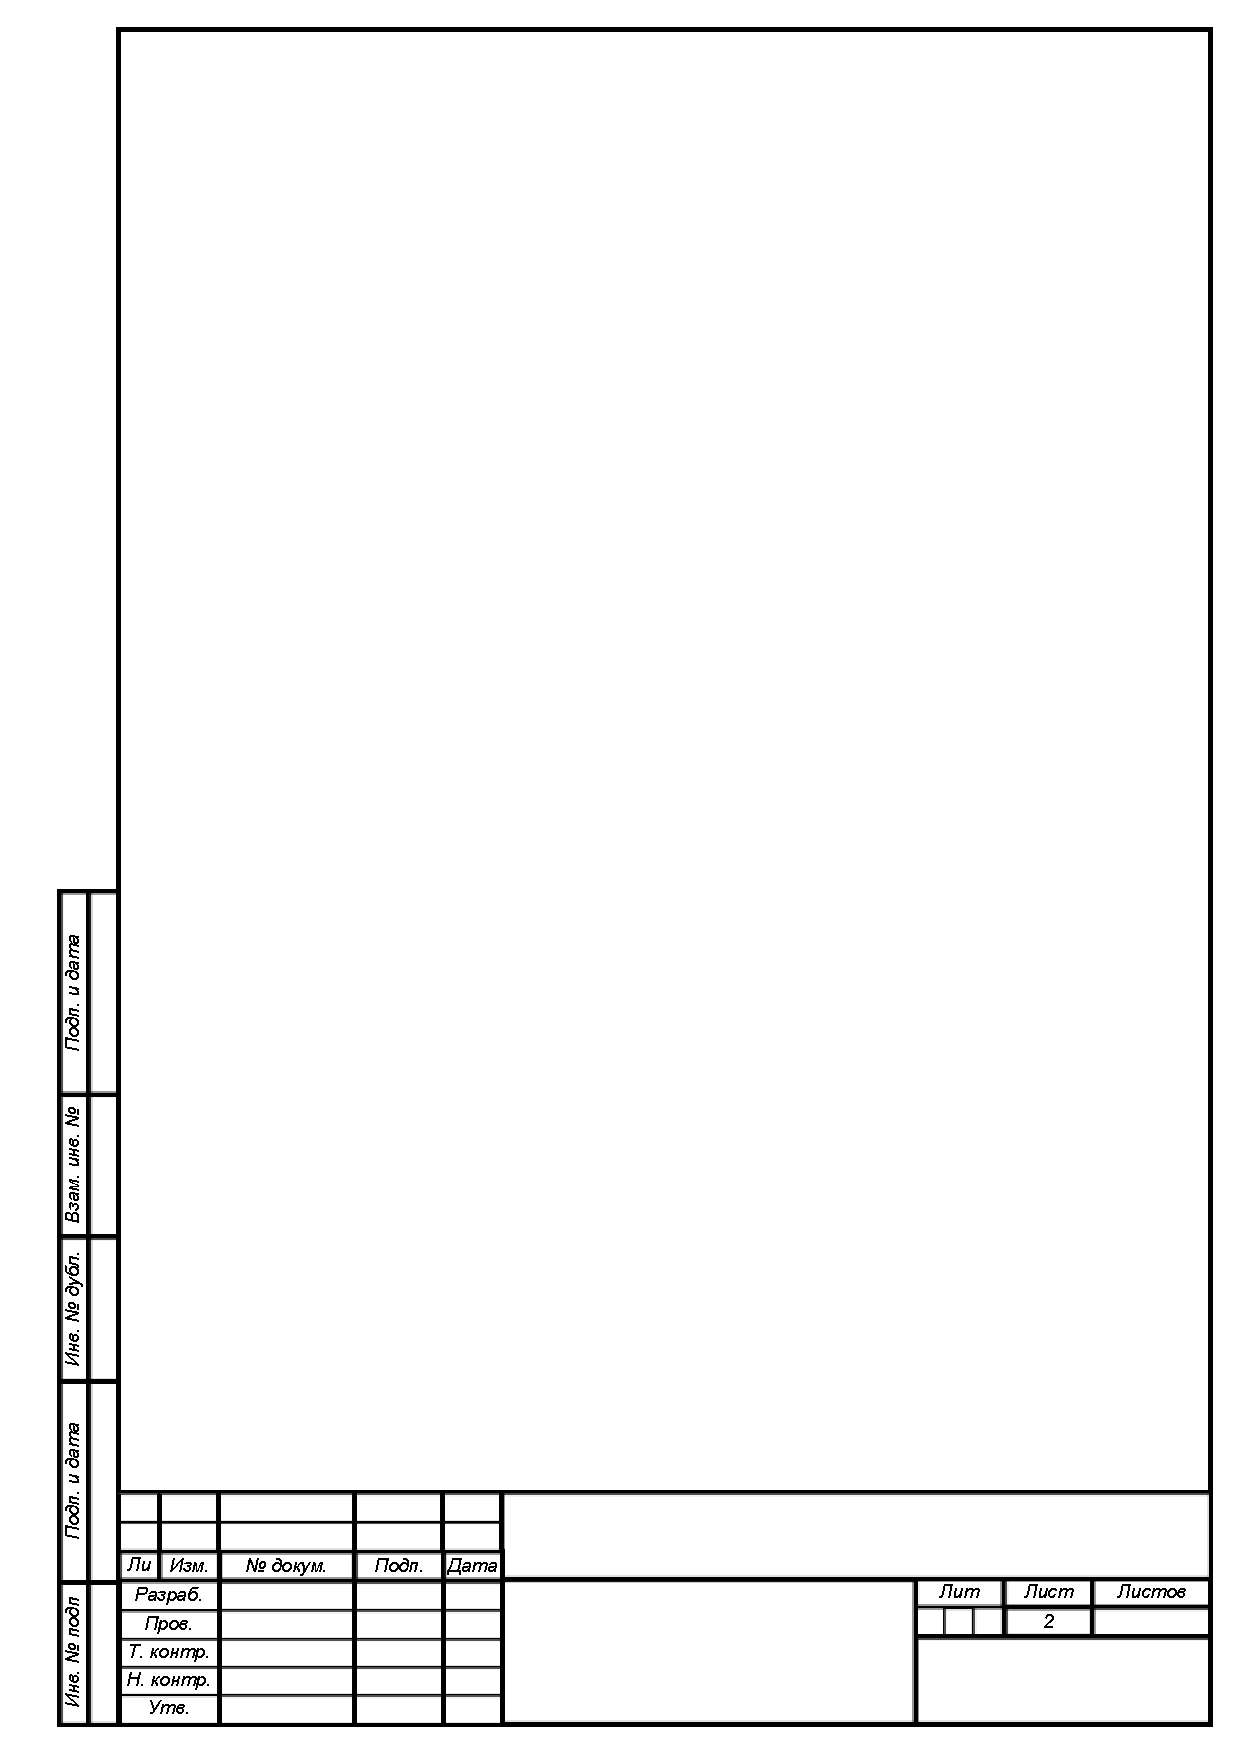
\includegraphics[width=\paperwidth,height=\paperheight]{./myimages/second.pdf}
		\vfill
}}}
		
		
\newcommand\BackgroundPicxx{
	\put(0,0){
		\parbox[b][\paperheight]{\paperwidth}{%
		\vfill
		\centering
		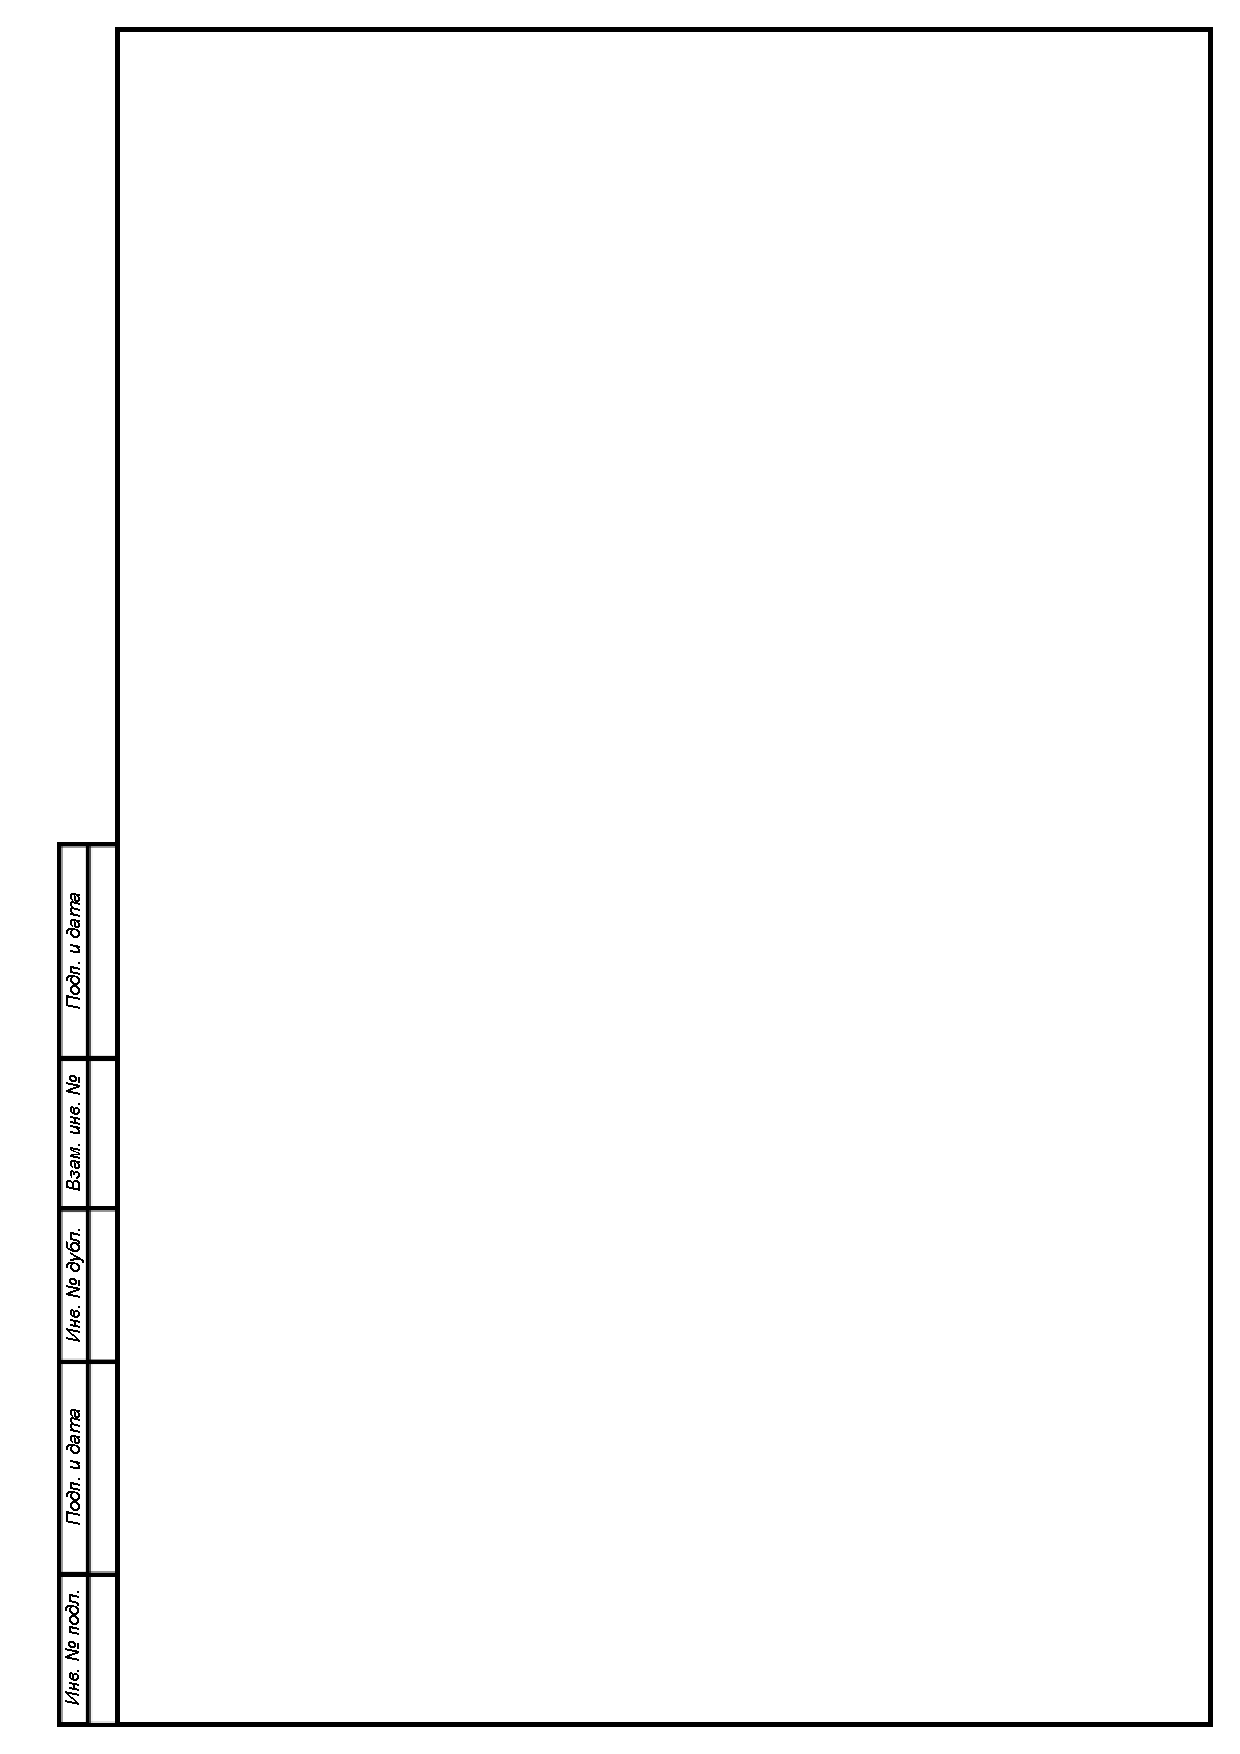
\includegraphics[width=\paperwidth,height=\paperheight]{./myimages/first.pdf}
		\vfill
}}}
				
\newcommand\BackgroundPicx{
	\put(0,0){
		\parbox[b][\paperheight]{\paperwidth}{%
		\vfill
		\centering
		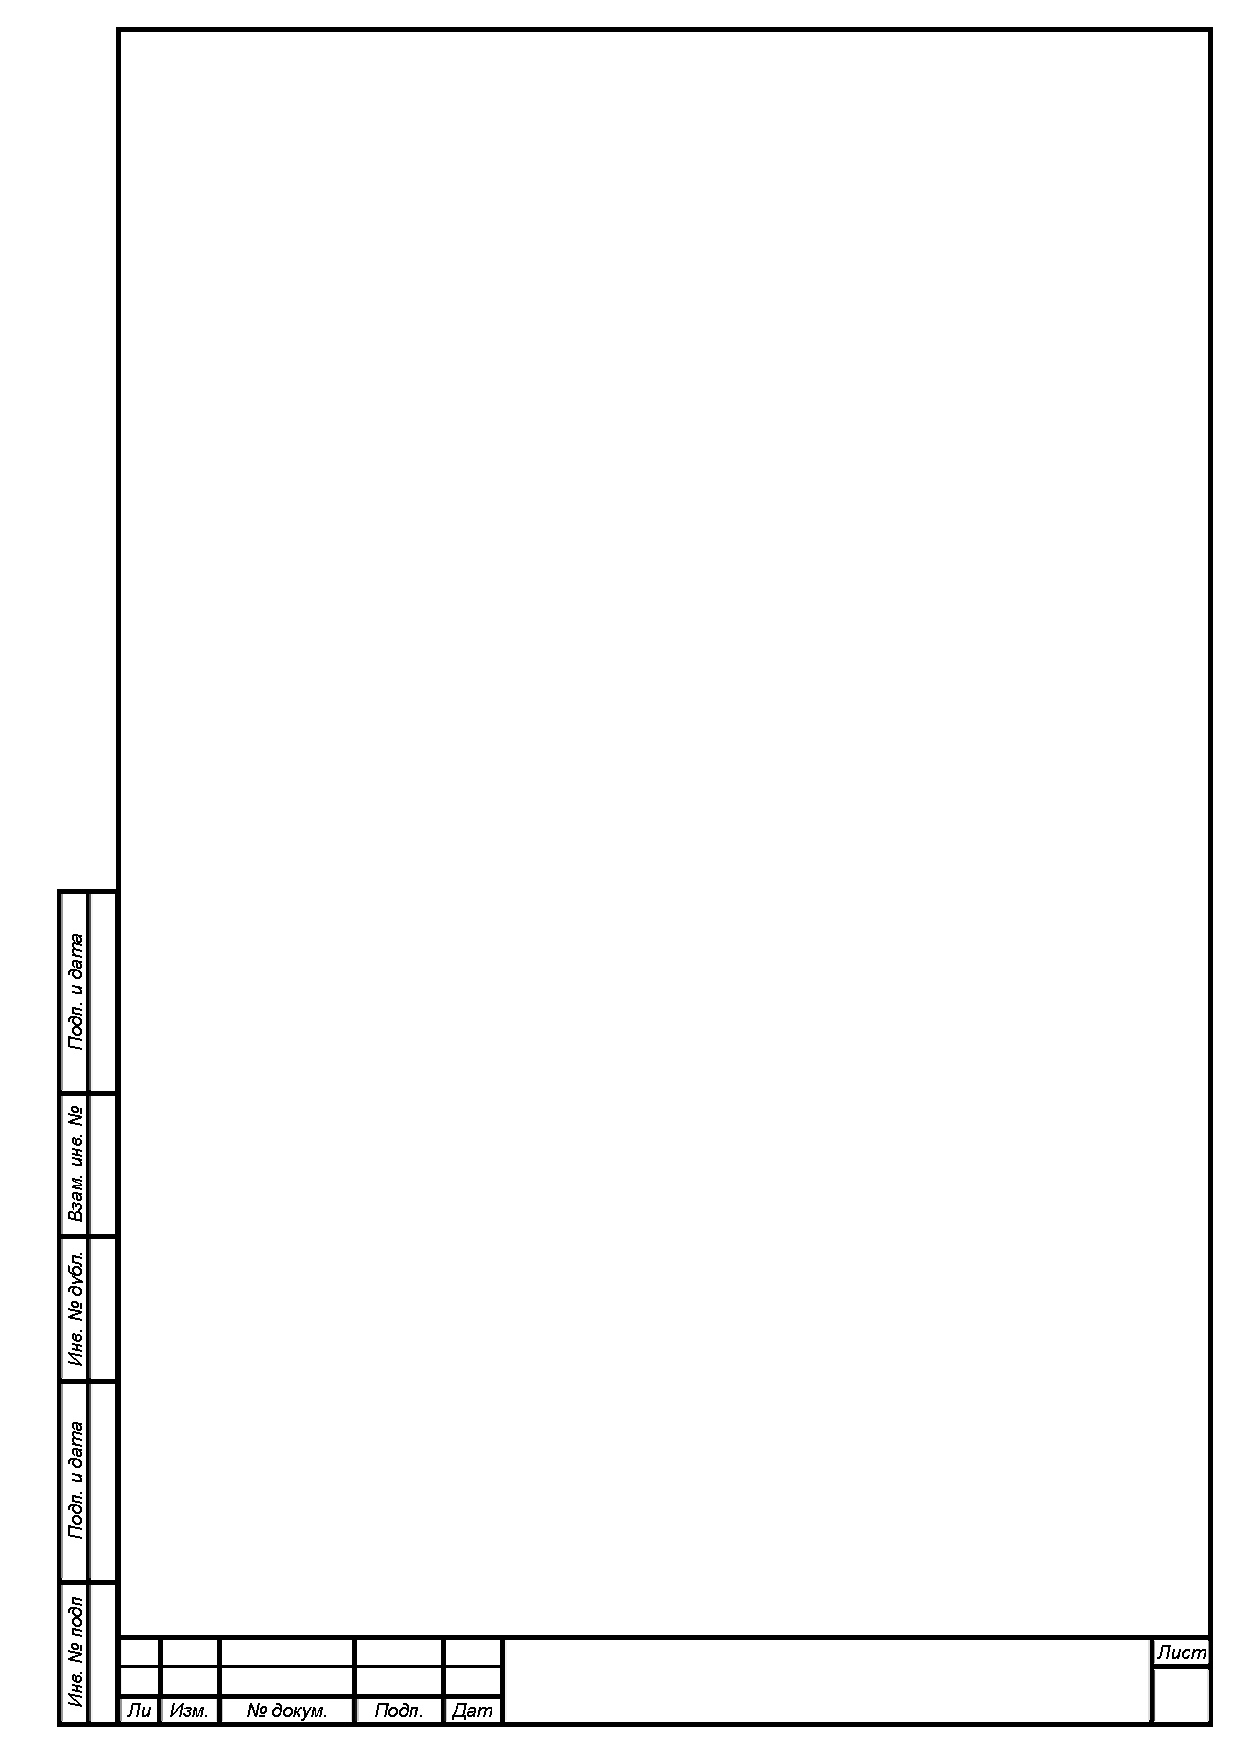
\includegraphics[width=\paperwidth,height=\paperheight]{./myimages/third.pdf}
		\vfill
}}}				
				
\begin{document}
	\AddToShipoutPicture*{\BackgroundPicxx}	
	%%% Переопределение именований %%%
\renewcommand{\abstractname}{Аннотация}
\renewcommand{\alsoname}{см. также}
\renewcommand{\appendixname}{Приложение}
\renewcommand{\bibname}{Литература}
\renewcommand{\ccname}{исх.}
\renewcommand{\chaptername}{}

\renewcommand{\contentsname}{Оглавление}
\renewcommand{\enclname}{вкл.}
\renewcommand{\figurename}{Рисунок}
\renewcommand{\headtoname}{вх.}
\renewcommand{\indexname}{Предметный указатель}
\renewcommand{\listfigurename}{Список рисунков}
\renewcommand{\listtablename}{Список таблиц}
\renewcommand{\pagename}{Стр.}
\renewcommand{\partname}{Часть}
\renewcommand{\refname}{Список литературы}
\renewcommand{\seename}{см.}
\renewcommand{\tablename}{Таблица}

%%% Основные сведения %%%

\newcommand{\thesisSpecialtyNumber}   {\texorpdfstring{{09.04.01}}{XX.XX.XX}}
\newcommand{\thesisSpecialtyTitle}    {\texorpdfstring{{Информатика и вычислительная техника}}{Название специальности}}
\newcommand{\thesisDegree}{{магистра}}
\newcommand{\thesisCity}  {{Нижний Новгород}}
\newcommand{\thesisYear} {{2016}}
\newcommand{\thesisOrganization} {{ФГОУ ВО Нижегородский государственный университет имени~Р.~Е.~Алексеева}}
			% Переопределение именований
	\thispagestyle{empty}%
\begin{center}%
	\MakeUppercase{\thesisOrganization}
\end{center}%
%
\vspace{0pt plus4fill} %число перед fill = кратность относительно некоторого расстояния fill, кусками которого заполнены пустые места
%
\vspace{0pt plus6fill} %число перед fill = кратность относительно некоторого расстояния fill, кусками которого заполнены пустые места
%
\vspace{0pt plus1fill} %число перед fill = кратность относительно некоторого расстояния fill, кусками которого заполнены пустые места
\begin{center}%

\begin{Large}
Лабораторная работа № 3\\
Технлогии распределенной обработки данных

Тема: Распараллеливание алгоритма с помощью библиотеки Concurrent
and Coordination Runtime

Вариант № 3	
\end{Large}
	
\end{center}%
%
\vspace{0pt plus5fill} %число перед fill = кратность относительно некоторого расстояния fill, кусками которого заполнены пустые места
\begin{flushright}%
Проверил:\\
Гай В. Е.

Выполнил:\\
Студент гр. 14-В-2\\
Носов А.В.
\end{flushright}%
%
\vspace{0pt plus4fill} %число перед fill = кратность относительно некоторого расстояния fill, кусками которого заполнены пустые места
\begin{center}%
	{\thesisCity~ \thesisYear}
\end{center}%
\newpage			% Титульный лист
	\AddToShipoutPicture*{\BackgroundPic}	
	\AddToShipoutPicture{\BackgroundPicx}
	\newcommand{\placetextbox}[3]{% \placetextbox{<horizontal pos>}{<vertical pos>}{<stuff>}
	\setbox0=\hbox{#3}% Put <stuff> in a box
	\AddToShipoutPictureFG*{% Add <stuff> to current page foreground
		\put(\LenToUnit{#1\paperwidth},\LenToUnit{#2\paperheight}){\vtop{{\null}\makebox[0pt][c]{#3}}}%
	}%
}%

\pagenumbering{gobble}
\fancyhf{}                          % Очищаем текущие значения

\chapter{Выполнение лабораторной работы}						

%\placetextbox{0.55}{0.1}{\Huge \textit{This is my text qweqwqweqw.}}%
%  {<width>}
%  [<left handle>,<top handle>]
%  (<leftmargin>,<topmargin>)

\begin{textblock}{10}[0,0](4.5, 10.9)
	\begin{center}
		\Large	Лабораторная работа № 3\\
	\end{center}
\end{textblock}

\begin{textblock}{5}[0,0](5, 11.5)
\begin{center}
\large	Распараллеливание алгоритма с помощью библиотеки CCR\\
\end{center}
\end{textblock}

\begin{textblock}{3}[0,0](12.5, 11.75)
	\pageref{LastPage}
\end{textblock}

\begin{textblock}{3}[0,0](11, 12.3)
	14-В-2
\end{textblock}
	
\section{Цель и вариант задания на лабораторную работу}	
	Целью данной лабораторной работы является получение представления о возможностях библиотеки Corrent and Coordination Runtime для организации параллельных вычислений.
	
	Вариант индивидуального задания:
	
	 Разработать алгоритм скалярного произведения n-мерных векторов

\section{Библиотека Concurrent and Coordination Runtime}
Библиотека Concurrent and Coordination Runtime (CCR) предназначена
для организации обработки данных с помощью параллельно и асинхронно
выполняющихся методов. Взаимодействие между такими методами
организуется на основе сообщений. Рассылка сообщений основана на
использовании портов.

Основные понятия CCR:

1) сообщение – экземпляр любого типа данных;

2) порт – очередь сообщений типа FIFO,
сообщение остаётся в порте пока не будут извлечено из очереди порта
получателем.
Отправка сообщения в порт:
p.Post(1);

3) получатель – структура, которая выполняет обработку сообщений.

Данная структура объединяет:

а) один или несколько портов, в которые отправляются сообщения;

б) методы, которые используются для обработки
сообщений;

в) логическое условие, определяющее ситуации, в которых
активизируется тот или иной получатель.

Получатели сообщений бывают двух типов: временные и постоянные. Временный получатель, обработав
сообщение, удаляется из списка получателей
сообщений данного порта.

4) процессом запуска задач управляет диспетчер. После выполнения
условий активации задачи (получение портом сообщения) диспетчер назначает задаче поток из пула
потоков, в котором она будет выполняться.

\chapter{Выполнение лабораторной работы}						

\pagenumbering{arabic}
\setcounter{page}{3}
\rfoot{\thepage}
\fancyfootoffset[L]{-6cm}
\setlength{\footskip}{1.3cm}
\cfoot[EO]{\fontsize{16}{12} \selectfont \textit{Лабораторная работа № 3} }

\section{Объявление структур данных}

Развмерность умножаемых векторов, количество компонент векторов, обрабатываемых в одном потоке, вектора a и b и переменные для хранения результата определены глобально:
\begin{figure}[h!]
	\center{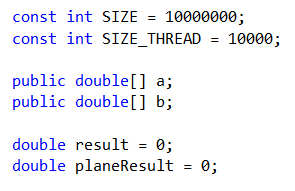
\includegraphics[scale = 0.5]{glob.png}}
\end{figure}

В методе Start() запускаются вычисления. Сначала в методе
выполняется вычисление скалярного скалярного произведения n-мерных векторов последовательным алгоритмом, затем та же задача решается с помощью
параллельных вычислений. Рассмотрим этот метод:
Выполняется инициализация структур данных:
\begin{figure}[h!]
	\center{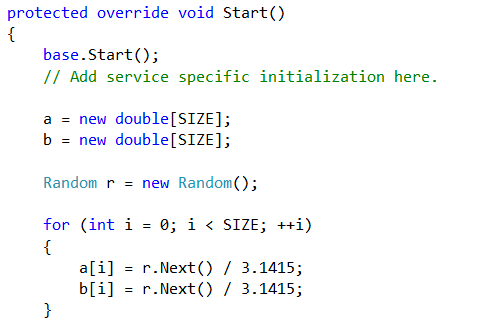
\includegraphics[scale = 0.5]{start.png}}
\end{figure}

\section{Последовательный алгоритм вычисления скалярного произведения n-мерных векторов }

 
 \begin{figure}[h!]
 	\center{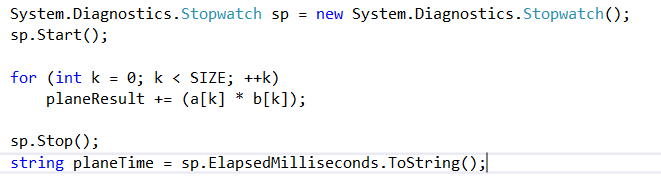
\includegraphics[scale = 0.5]{seq.png}}
 \end{figure}
 
\clearpage

\section{Параллельный алгоритм вычисления скалярного произведения n-мерных векторов}

Параллельная обработка выполняется с помощью запуска нескольких
копий вычислительного метода. Каждая копия метода выполняет
обработку определённой части исходных данных. Для описания задания
для каждого метода используется класс InputData:

\center{public double[] a;\\
public double[] b;\\}
Поле а класса хранит компоненты векторов. Поля рассчитываются с помощью экземпляра вычислительного
метода.

\begin{figure}[h!]
	\center{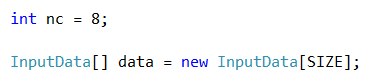
\includegraphics[scale = 0.5]{param.png}}
\end{figure}

Далее, задаются исходные данные для каждого экземпляра
вычислительного метода:

\begin{figure}[h!]
	\center{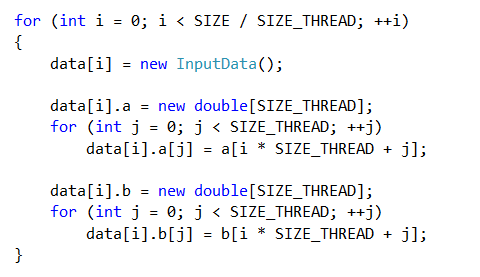
\includegraphics[scale = 0.5]{is_data.png}}
\end{figure}

Создаётся диспетчер с пулом из 8 потоков и описывается порт, в который каждый экземпляр метода Sort() отправляет сообщение после завершения вычислений:

\begin{figure}[h!]
	\center{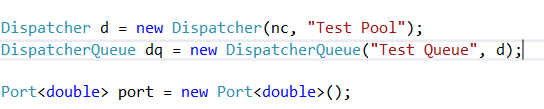
\includegraphics[scale = 0.5]{disp.png}}
\end{figure}

Метод Arbiter.Activate помещает задачи в очередь диспетчера:

\begin{figure}[h!]
	\center{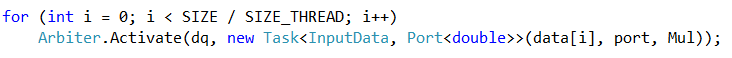
\includegraphics[scale = 0.5]{arb.png}}
\end{figure}

Первый параметр метода Arbiter.Activate – очередь диспетчера,
который будет управлять выполнением задачи, второй параметр –
запускаемая задача.

С помощью метода Arbiter.MultipleItemReceive запускается задача
(приёмник), которая обрабатывает сообщения:

\begin{figure}[h!]
	\center{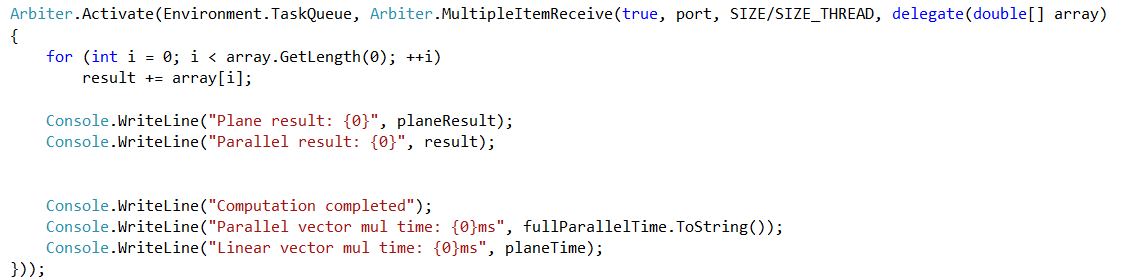
\includegraphics[scale = 0.5]{act.png}}
\end{figure}

Приёмник используется для определения момента окончания
вычислений. Он сработает только после того, как в порт p придут все сообщения. В делегат, описанный в приёмнике,  включим действия,
которые будут выполнены после завершения процесса сортировки в каждом из потоков. Такими действиями является вывод результата, а также подсчет результатов интегрирования подотрезков.

Метод Mul() выполняет скалярное произведение:

\begin{figure}[h!]
	\center{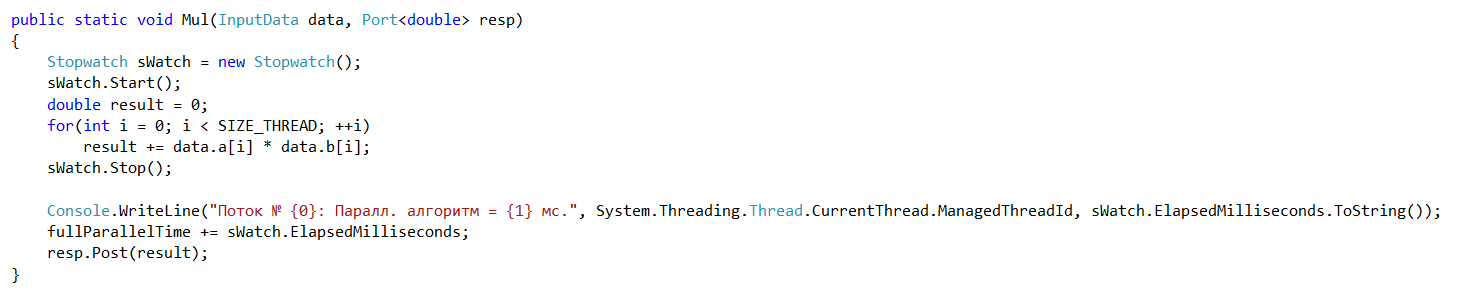
\includegraphics[scale = 0.5]{mul.png}}
\end{figure}

Метод Mul() имеет два параметра:
1) индекс, хранящий значение элемента массива, который определяет
параметры, передаваемые на вход метода;
2) порт завершения, в который отправляется экземпляр класса double после
завершения вычислений.
После завершения вычислений метод Mul отправляет в порт p
значение экземпляра класса double, который необходим определения времени завершения вычислений.
Результат вычислений показан на рисунке:

\begin{figure}[h!]
	\center{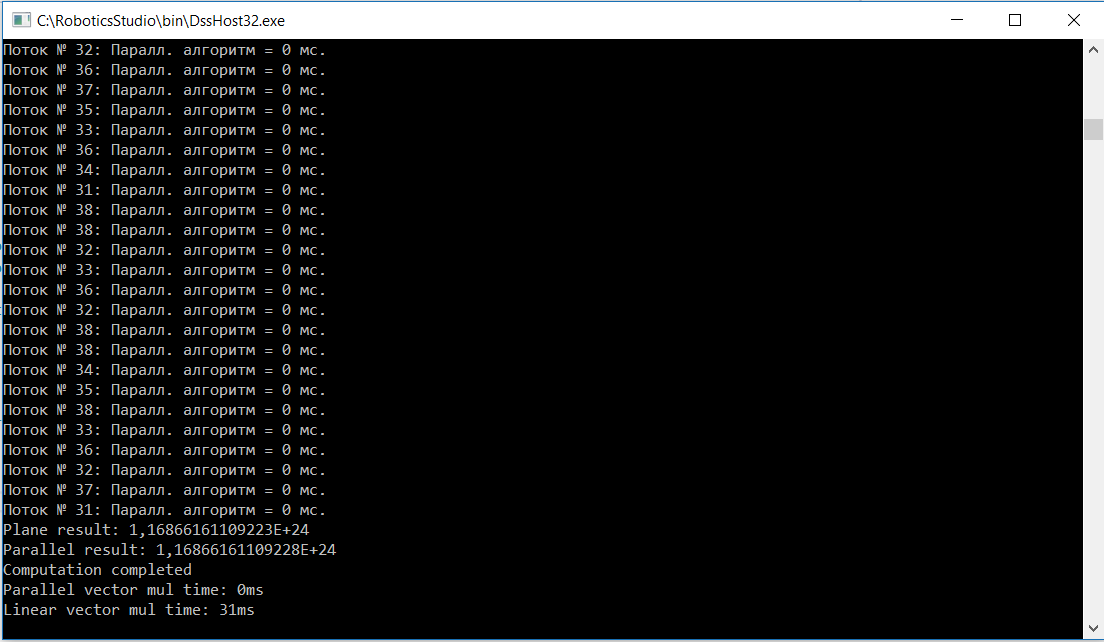
\includegraphics[scale = 0.3]{scr.png}}
\end{figure}


\section*{Выводы}
Таким образом, в ходе данной лабораторной работы были изучены и освоены на практике возможности библиотеки Corrent and Coordination Runtime для организации параллельных вычислений. Разработаны последовательный и параллельный алгоритмы вычисления скалярного произведения n-мерных векторов. Исходя из работы программы можно сделать вывод о том, что время выполнения последовательного алгоритма примерно в несколько раз больше, чем время выполнения параллельного алгоритма, также результаты при последовательном и параллельном алгоритмах одинаковые, то есть программа работает правильно.
\end{document}

	% Введение
	\chapter*{Заключение}						% Заголовок
\addcontentsline{toc}{chapter}{Заключение}	% Добавляем его в оглавление

Основные результаты работы заключаются в следующем.
\begin{enumerate}
	
	\item В данной работе был представлен и обоснован пример разработки моделей монауральной локализации источника звука. Предварительно проведен анализ исследований и результатов работы существующих систем, выполняющих схожие задачи.
	
	\item В диссертации исследованы следующие задачи
	
	\begin{enumerate}
		\item Разработана система локализации источника звука, было выполнено построение ее модели и решение с помощью необходимых методов.
		\item Разработана программная реализация модели системы
		\item Выполнено тестирование, включающее в себя проведение экспериментов с реализованной моделью, поиск алгоритма ее работы, дающего наилучший результат, а так же сравнение конечных результатов с аналогами.\\
	\end{enumerate}
	
	  \item В работе адаптирована теория активного восприятия, применительно к обработке и анализу звуковых сигналов
	  
	  \item Все представленные в работе методы реализованы в виде программного обеспечения, способного работать на большом количестве распространенных персональных вычислительных машин.
	  
	  \item По результатам исследований опубликовано несколько статей.
	  
  
\end{enumerate}
В результате выполнения работы были получены знания в областях исследований, имеющих непосредственное отношение к теме магистерской работы: машинном обучении, анализу сигналов, математическом моделировании, улучшены практические навыки разработки программного обеспечения. Получен опыт обоснованного выбора и использования программных продуктов для решения поставленных задач, самостоятельного изучения новых методов исследований и проведения научных исследований в соответствии с тематикой задания. На практике выполнена разработка программной системы, решающей поставленную задачу, а так же проведено ее тестирование с анализом полученных результатов и их сравнением с результатами известных исследований в данной области. Обозначены перспективы дальнейшего модифицирования и развития и системы. 

\clearpage		% Заключение
\end{document}